\documentclass[handout]{beamer}

\usepackage{fontspec} 
% \usepackage{lsp-makros}
\useoutertheme{lsp}

\usepackage{lsptitle}

\def\two@digits#1{\ifnum#1<10 0\fi\number#1}
\def\mytoday{\two@digits{\number\day}.\two@digits{\number\month}.\number\year}


\usepackage{xspace,multicol}
\newcommand{\latex}{\LaTeX\xspace}
\usepackage{tikz}


\newcounter{lastpagemainpart}
\footnotesep0pt
\renewcommand{\footnoterule}{}
\usefootnotetemplate{
  \noindent
  \insertfootnotemark\insertfootnotetext}

\let\beamerfn=\footnote
\renewcommand{\footnote}[1]{%
\let\oldfnsize=\footnotesize%
\let\footnotesize=\tiny%
\beamerfn<\thebeamerpauses->{#1}%
\let\footnotesize=\oldfnsize}


\date{\today}

\usepackage{eurosym}  
 
\renewcommand{\centerline}[1]{\hfill#1\hfill\hfill\mbox{}}


\title{Review of peer review}
% \institute{FU Berlin}
\author[LangSci]{Sebastian Nordhoff}



\begin{document}
\lspbeamertitle



\frame{
\frametitle{Review typology}
%   \includegraphics[height=.2\textheight]{./path/to/graphicsfile}
  \begin{itemize}
    \item  scarce: grants, conferences
    \item  not-so-scarce: journal articles, books
    \item hypothesis: reviews for scarce goods create more frustration and are more often perceived as ``unfair''.
  \end{itemize}
}

\section{Reviewer fatigue}
\frame{
\frametitle{Is there reviewer fatigue?}
  \begin{itemize}
    \item are too many reviews solicited from individual researchers? 
    \item probably differences between books, journals, abstracts, grants
    \item LangSci series editors do not report any particular problems in recruiting reviewers
    \item getting reviewers to submit reviews in time requires some nagging, but seems feasible
  \end{itemize}
}


\section{Reviewer recognition}
 
\frame{
\frametitle{Reviewer recognition}
  \begin{itemize}
    \item In an competitive job market, researchers have to choose what to devote their time on
    \begin{itemize}
      \item articles
      \item data curation 
      \item reviewing
      \item {\dots}
    \end{itemize}
    \item articles figure prominently on your CV, data curation less, reviews even less so 
    \item reviews don't really offer return on your time investment
    \item ``I would like to thank two anonymous reviewers for helpful comments''
    \begin{itemize}
      \item does not really help your job prospects
    \end{itemize}
  \end{itemize}
} 

\frame{
\frametitle{Acknowledging reviewers}
%   \includegraphics[height=.2\textheight]{./path/to/graphicsfile}
  \begin{itemize}
    \item not at all
    \item  once a year in summary note in the journal frontmatter
    \item review statement ``book reviewed by John Goldsmith and Mark Gibson"
    \item open review: full review is available for inspection together with the book
    \begin{itemize}
      \item also said to improve civility and constructiveness in reviews
    \end{itemize}
    \item Publons: service which aggregates confirmed reviews.
    \begin{itemize}
    \item very commodified 
    \end{itemize}
  \end{itemize}
}

\frame{
\frametitle{More on open review}
%   \includegraphics[height=.2\textheight]{./path/to/graphicsfile}
  \begin{itemize}
    \item Ross-Hellauer T. What is open peer review? A systematic review. F1000Research 2017, 6:588
\url{https://doi.org/10.12688/f1000research.11369.2}
\item shortcomings of traditional closed peer review
\begin{itemize}
  \item reviewers have only weak levels of agreement, only slightly greater than chance 
  \item ``Peters and Ceci’s classic study found that eight out of twelve papers were rejected for methodological flaws when resubmitted to the same journals in which they had already been published''
  \item ``Reviewers often fail to detect major methodological failings''
  \item ``The global costs of reviewers’ time estimated at £1.9bn in 2008''
\end{itemize}
  \end{itemize}
}

\frame{
\frametitle{Even more on open review}
%   \includegraphics[height=.2\textheight]{./path/to/graphicsfile}
  \begin{itemize}
    \item  Tennant JP, Dugan JM, Graziotin D et al. A multi-disciplinary perspective on emergent and future innovations in peer review. F1000Research 2017, 6:1151
(\url{https://doi.org/10.12688/f1000research.12037.3})  
\item ``we have little or no evidence that peer review ‘works,’ but we have lots of evidence of its downside''
\item ``These dysfunctional issues should be deeply troubling to those who hold peer review in high regard as a `gold standard'{}''.
  \end{itemize}
}

\frame{
\frametitle{Peer review: the editor's\\ decision}
%   \includegraphics[height=.2\textheight]{./path/to/graphicsfile}
  \begin{itemize}
    \item  Based on the available empirical evidence, we should actually stop closed peer review right away
    \begin{itemize}
      \item expensive
      \item unreliable 
      \item cumbersome
      \item slowing down research
    \end{itemize}
  \end{itemize}
}

\frame{
\frametitle{Is closed peer review going to go away any time soon?}
%   \includegraphics[height=.2\textheight]{./path/to/graphicsfile}
  \begin{itemize}
    \item grants: unlikely because conflict of interest
    \item conferences: unlikely because conflict of interest 
    \item books: unlikely because no crowd
    \item journal articles: possibly
  \end{itemize}
}

\frame{
\frametitle{Open peer review in\\ \mbox{Atmospheric chemistry and physics}}
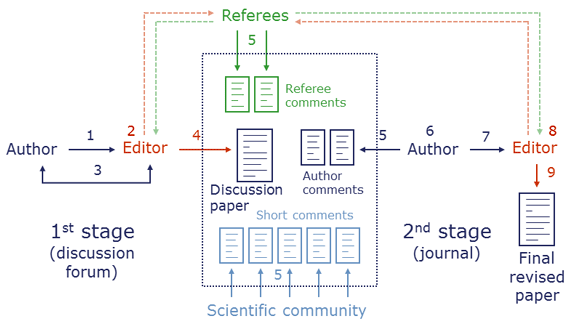
\includegraphics[height=\textheight]{acp-peerreview.png}
}
\end{document}

